\documentclass[11pt,a4paper]{article}

\usepackage[margin=2.15cm]{geometry}
\usepackage[T1]{fontenc}
\usepackage[utf8]{inputenc}
\usepackage{lmodern}
\usepackage{microtype}
\usepackage{amsmath,amssymb,mathtools,bm}
\usepackage{booktabs,tabularx,longtable,array,multirow}
\usepackage{graphicx}
\usepackage{caption,subcaption}
\usepackage{enumitem}
\usepackage{xcolor}
\usepackage{hyperref}
\usepackage{cleveref}
\usepackage[numbers,sort&compress]{natbib}
\usepackage{fancyhdr}
\usepackage{titlesec}
\usepackage{float}
\usepackage{siunitx}
\usepackage{url}
\usepackage[most]{tcolorbox}
\usepackage{tikz}
\usetikzlibrary{arrows.meta,positioning,fit,calc,shapes.geometric}

\definecolor{deepblue}{RGB}{28,63,105}
\definecolor{deepgreen}{RGB}{38,105,79}
\definecolor{deeporange}{RGB}{170,92,20}
\definecolor{softblue}{RGB}{232,241,250}
\definecolor{softgreen}{RGB}{235,247,240}
\definecolor{softorange}{RGB}{253,243,226}
\definecolor{softred}{RGB}{252,235,235}
\definecolor{softgray}{RGB}{245,246,248}
\definecolor{deepred}{RGB}{145,52,52}

\hypersetup{
  colorlinks=true,
  linkcolor=deepblue,
  citecolor=deepgreen,
  urlcolor=deeporange,
  pdftitle={Geometry-MMALS G1: Status, Evidence, and Research Perspective},
  pdfauthor={Guillaume Harbonnier}
}

\pagestyle{fancy}
\fancyhf{}
\lhead{Geometry-MMALS G1}
\rhead{Reviewer-oriented status report}
\cfoot{\thepage}
\setlength{\headheight}{14pt}

\titleformat{\section}{\Large\bfseries\color{deepblue}}{\thesection}{0.8em}{}
\titleformat{\subsection}{\large\bfseries\color{deepgreen}}{\thesubsection}{0.8em}{}
\titleformat{\subsubsection}{\normalsize\bfseries\color{deeporange}}{\thesubsubsection}{0.8em}{}

\setlist[itemize]{leftmargin=1.5em,itemsep=2pt,topsep=3pt}
\setlist[enumerate]{leftmargin=1.7em,itemsep=3pt,topsep=3pt}
\renewcommand{\arraystretch}{1.15}
\newcolumntype{Y}{>{\raggedright\arraybackslash}X}
\newcolumntype{C}{>{\centering\arraybackslash}X}
\newcommand{\MMALS}{\textsc{MMALS}}
\newcommand{\R}{\mathbb{R}}
\newcommand{\E}{\mathbb{E}}
\newcommand{\loss}{\mathcal{L}}
\newcommand{\norm}[1]{\left\lVert #1 \right\rVert}

\newtcolorbox{summarybox}{
  colback=softblue,colframe=deepblue!45,boxrule=0.6pt,arc=2pt,
  left=8pt,right=8pt,top=7pt,bottom=7pt
}
\newtcolorbox{positivebox}{
  colback=softgreen,colframe=deepgreen!45,boxrule=0.6pt,arc=2pt,
  left=8pt,right=8pt,top=7pt,bottom=7pt
}
\newtcolorbox{warningbox}{
  colback=softorange,colframe=deeporange!50,boxrule=0.6pt,arc=2pt,
  left=8pt,right=8pt,top=7pt,bottom=7pt
}
\newtcolorbox{criticalbox}{
  colback=softred,colframe=deepred!50,boxrule=0.6pt,arc=2pt,
  left=8pt,right=8pt,top=7pt,bottom=7pt
}

\begin{document}

\begin{titlepage}
\centering
\vspace*{1.1cm}
{\Huge\bfseries\color{deepblue} Geometry-MMALS G1\par}
\vspace{0.25cm}
{\LARGE Status, Evidence, Limitations, and Research Perspective\par}
\vspace{0.45cm}
{\large A reviewer-oriented arXiv-style technical report\par}
\vspace{1.1cm}
{\Large Guillaume Harbonnier\par}
\vspace{0.2cm}
{\normalsize Independent MMALS research program\par}
\vspace{0.15cm}
{\normalsize \href{https://github.com/gharbonnier78/geometry-mmalls-g1}{github.com/gharbonnier78/geometry-mmalls-g1}\par}
\vspace{0.7cm}
{\normalsize Evidence snapshot: Geometry-MMALS G1 v1.0.6, seed 0, development protocol\par}
{\normalsize June 2026\par}
\vfill
\begin{minipage}{0.90\textwidth}
\small
\textbf{Epistemic status.} This report summarizes the conceptual program, implementation history, and the strongest evidence available through v1.0.6. It is not a qualification paper. The current empirical evidence is a single development seed on controlled RotatedMNIST. C0 protocol integrity is supported; C1 contains candidate evidence for route geometry; C2--C6 remain unqualified or failed. No claim of quantum computation, quantum advantage, backward transfer, universal intelligence, or domain-general geometry is made.
\end{minipage}
\vfill
\end{titlepage}

\begin{abstract}
Geometry-MMALS G1 investigates whether a continual-learning mixture of functional hosts can acquire an internal geometry that is more than a projection of audit variables: a geometry of inferred contexts, routing distributions, host transformations, synthesized representations, and their transport through learning time. The program was designed around a strict evidence ladder: descriptive order, predictive interpolation, causal intervention, functional specialization, continual transport, and operational utility. This reviewer-oriented report consolidates the conceptual model, mathematical definitions, protocol evolution from v1.0.0 to v1.0.6, and the latest controlled development evidence.

The strongest current result is narrow but reproducible within the seed-0 archive: under matched initialization, matched paired compute, and source-paired bootstrap analysis, the explicit geometry objective increases trained-angle route order by $\Delta\rho=0.0558$ with a 95\% interval $[0.0407,0.0713]$, and improves synthesis order by $0.0160$ with interval $[0.0091,0.0226]$. It does not improve context order, and it yields almost no predictive advantage. A small retention anchor produces the main operational gains, while adaptive routing does not reliably outperform uniform or learned-static mixtures. Router interventions show that direct sensory features dominate inferred context by approximately an order of magnitude. Counterbalanced curricula sharing the same final task still produce large performance variation, revealing substantial order sensitivity. Causal specificity remains below the preregistered threshold, host specialization is not reproducibly established, and functional memory transport has not yet been tested.

The appropriate reviewer conclusion is therefore not rejection of the geometric hypothesis, nor acceptance of a completed continual-learning method. The evidence supports a serious, falsifiable research program with one candidate empirical contribution: geometry regularization measurably organizes route space. The decisive next question is whether this organization can be made context-mediated, causally specific, curriculum-robust, and operationally superior across seeds and a second controlled transformation.
\end{abstract}

\begin{summarybox}
\textbf{Reviewer recommendation in one sentence.} The work is credible as a protocol-and-status paper or perspective, but an empirical results submission requires major revision: multi-seed confirmation, genuine context mediation, static-route superiority tests, counterbalanced curriculum robustness, and a secondary dataset.
\end{summarybox}

\tableofcontents
\newpage

\section{Purpose of this report}

This document is written for a technically demanding reviewer who needs to answer four questions:

\begin{enumerate}
\item Is the research question meaningful and distinct from standard mixture-of-experts or continual-learning evaluation?
\item Which claims are already supported, which are merely promising, and which have failed?
\item Are the negative results scientifically useful, or do they expose a fundamentally incoherent program?
\item What exact evidence would be required for a publishable empirical paper?
\end{enumerate}

The report is deliberately more critical than a project overview. It treats implementation corrections, failed controls, and confounds as part of the scientific record rather than as details to hide.

\section{Research question and conceptual contribution}

\subsection{From audit geometry to functional geometry}

Earlier MMALS experiments used vectors of observable indicators---accuracy, retention, cost, drift, host contribution, route confidence, and auditability---to compare candidate traces and select policies under changing goals. This is useful, but it is an \emph{external geometry of control}. It does not establish that the learning system has organized its own representations or functions geometrically.

Geometry-MMALS G1 instead studies the internal chain

\begin{equation}
 x \longrightarrow z_0 \longrightarrow c \longrightarrow r
 \longrightarrow \{g_h(z_0)\}_{h=1}^{H}
 \longrightarrow z_M \longrightarrow \hat y,
\end{equation}

where $z_0$ is a frozen sensory representation, $c$ is inferred context, $r$ is a route on the host simplex, $g_h$ is host $h$'s transformation, and $z_M$ is the synthesized representation.

The central question is:

\begin{quote}
Does a continual-learning MMALS system learn a stable relation among context, route, host function, and memory that preserves known transformation order, predicts unseen contexts, supports causal control, and improves a concrete objective?
\end{quote}

This differs from standard MoE work, where routing is usually evaluated by task performance, sparsity, load balancing, or scale efficiency \citep{shazeer2017moe,fedus2022switch}. It also differs from purely descriptive representation analysis: a two-dimensional projection is not accepted as evidence unless it survives predictive, causal, and operational tests.

\subsection{Why geometry is not merely parameter distance}

Weight-space distances are not reliable functional distances because neural networks admit permutations, rescalings, and other symmetries that can alter parameters while preserving behavior \citep{dinh2017sharp}. G1 therefore prioritizes:

\begin{itemize}
\item distances among representations of the same source under controlled transformations;
\item information geometry on route distributions;
\item functional distances measured by host outputs and ablations;
\item alignment and transport across continual-learning stages.
\end{itemize}

This is related to information geometry \citep{amari1998natural}, learned latent geometry \citep{arvanitidis2018latent,shao2018riemannian}, and geometric deep learning \citep{bronstein2021geometric}, but the proposed object is specifically a \emph{route-function geometry under continual change}.

\subsection{Potential conceptual novelty}

The most defensible novelty is not a new optimizer or a claim that ``intelligence is geometry.'' It is the conjunction of five design choices:

\begin{enumerate}
\item a frozen sensory boundary that prevents perceptual geometry from being attributed automatically to MMALS;
\item same-source cross-context measurement, which separates transformation geometry from class identity;
\item an evidence ladder from description to causal and operational utility;
\item ecological host specialization defined by function and ablation rather than route frequency;
\item continual geometric transport as an explicit future claim rather than an implicit synonym for retention.
\end{enumerate}

\section{Mathematical model}

\subsection{Route geometry}

For $H$ hosts, a route is a probability vector

\begin{equation}
 r(x) \in \Delta^{H-1}, \qquad r_h\ge 0, \qquad \sum_h r_h=1.
\end{equation}

Evaluation uses the Fisher--Rao distance on the simplex,

\begin{equation}
 d_{\mathrm{FR}}(r_i,r_j)
 =2\arccos\left(\sum_{h=1}^{H}\sqrt{r_{ih}r_{jh}}\right).
\end{equation}

Training uses the monotonic chordal distance in square-root coordinates to avoid the derivative singularity of $\arccos$ near identical routes. For source $s$ observed at factors $u_a$ and $u_b$, the paired objective encourages route distance to reflect factor distance:

\begin{equation}
 \loss_{\mathrm{geo}}
 = \E_s\sum_{a<b}
 \left(d_{\sqrt\Delta}(r_{s,a},r_{s,b})-	au(u_a,u_b)\right)^2
 + \lambda_{\mathrm{far}}\loss_{\mathrm{margin}}.
\end{equation}

The current G1-A protocol is supervised by the known rotation angle during training; the angle is not supplied to the deployable router at inference. This is a controlled grounding experiment, not a claim of unsupervised manifold discovery.

\subsection{Synthesis and host function}

The synthesized representation is

\begin{equation}
 z_M(x)=\sum_{h=1}^{H} r_h(x)\,g_h(z_0(x)).
\end{equation}

A host is not called specialized because it receives route mass. Its functional contribution is estimated by route-renormalized ablation:

\begin{equation}
 \Delta_h(x)=\log p(y\mid x)-\log p_{-h}(y\mid x).
\end{equation}

A credible specialization claim requires localized positive contribution, reproducibility across seeds after host matching, and stability through learning stages. Raw dominance is explicitly insufficient.

\subsection{Retention anchor}

The current anchor is controlled rehearsal over previously seen views already present in a paired batch:

\begin{equation}
 \loss = \loss_{\mathrm{current}}
 + \lambda_{\mathrm{anchor}}\loss_{\mathrm{old\ views}}
 + \lambda_{\mathrm{geo}}\loss_{\mathrm{geo}}
 + \lambda_{\mathrm{div}}\loss_{\mathrm{host}}.
\end{equation}

It is not yet MMALS reconstructive memory or synthetic compiled memory. Its purpose is to test whether functional evidence stabilizes geometric organization.

\subsection{Causal specificity}

A context direction $t_c$ associated with increasing angle is estimated from trained contexts. The route response is projected onto a route-angle direction $t_r$. The causal specificity ratio is

\begin{equation}
 \mathrm{CSR}
 =\frac{|\E\langle \Delta\sqrt r(t_c),t_r\rangle|}
 {\E_{q\perp t_c}|\langle\Delta\sqrt r(q),t_r\rangle|}.
\end{equation}

The pilot gate requires CSR $>1.5$, a bootstrap lower bound above $1.0$, correct orientation, monotonic magnitude, and preserved class identity.

\section{Evidence ladder and claim discipline}

\begin{figure}[H]
\centering
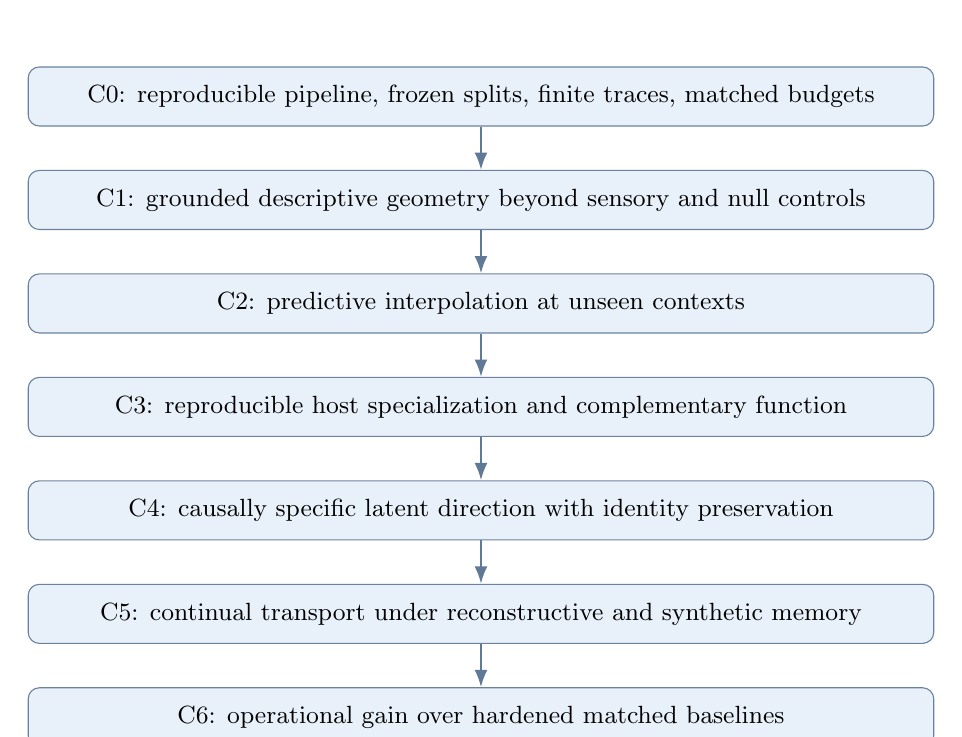
\begin{tikzpicture}[
 node distance=0.55cm,
 every node/.style={font=\small},
 box/.style={draw=deepblue!65,rounded corners,fill=softblue,minimum width=11.5cm,minimum height=0.75cm,align=center},
 arr/.style={-{Latex[length=2.2mm]},thick,deepblue!70}
]
\node[box] (c0) {C0: reproducible pipeline, frozen splits, finite traces, matched budgets};
\node[box,below=of c0] (c1) {C1: grounded descriptive geometry beyond sensory and null controls};
\node[box,below=of c1] (c2) {C2: predictive interpolation at unseen contexts};
\node[box,below=of c2] (c3) {C3: reproducible host specialization and complementary function};
\node[box,below=of c3] (c4) {C4: causally specific latent direction with identity preservation};
\node[box,below=of c4] (c5) {C5: continual transport under reconstructive and synthetic memory};
\node[box,below=of c5] (c6) {C6: operational gain over hardened matched baselines};
\draw[arr] (c0)--(c1);\draw[arr] (c1)--(c2);\draw[arr] (c2)--(c3);
\draw[arr] (c3)--(c4);\draw[arr] (c4)--(c5);\draw[arr] (c5)--(c6);
\end{tikzpicture}
\caption{Geometry-MMALS evidence ladder. Passing a lower level does not imply the next one.}
\label{fig:ladder}
\end{figure}

The ladder is the strongest methodological aspect of the program. It prevents visually attractive embeddings from becoming geometric claims, and prevents geometric order from being equated automatically with useful continual learning. It also makes negative results informative: a model can pass route-ordering tests while failing causality or utility.

\section{Research history: what each revision corrected}

\begin{longtable}{p{1.4cm}p{4.0cm}p{8.2cm}}
\toprule
\textbf{Version} & \textbf{Question} & \textbf{Outcome and scientific lesson}\\
\midrule
\endfirsthead
\toprule
\textbf{Version} & \textbf{Question} & \textbf{Outcome and scientific lesson}\\
\midrule
\endhead
v1.0.0 & Can functional geometry be specified? & Conceptual article, internal/external geometry distinction, evidence ladder, RotatedMNIST blueprint.\\
v1.0.1 & Can release claims and gates be audited? & C0-only status, pilot thresholds, notation bridge, dual-memory contracts, and explicit supervised G1-A labeling.\\
v1.0.2 & Can the route loss train without numerical failure? & Fisher--Rao derivative instability identified; stable square-root-simplex training and finite-value guards added.\\
v1.0.3 & Does a geometry batch contain actual cross-angle evidence? & Same-source multi-angle batches introduced. First informative development result; exposed initialization and compute confounds.\\
v1.0.4 & Does geometry add value under matched initialization and compute? & Geometry improved route alignment modestly; retention anchor improved function; context bypass and static-route questions emerged.\\
v1.0.5 & Is routing truly context-mediated, and does curriculum order matter? & Standard router was dominated by direct sensory input; static-like routing could outperform it; curriculum effects were large but terminal-task confounded.\\
v1.0.6 & Does adaptive routing beat static mixtures, and do curriculum effects survive same-final-task balancing? & Release integrity, uniform/learned-static controls, source-paired mediation intervals, and four counterbalanced curricula. Strong route geometry effect; no reliable adaptive or predictive advantage.\\
\bottomrule
\end{longtable}

This history matters for review because the current conclusions were not selected after one favorable run. Each revision was triggered by a failure or confound, and the resulting controls often weakened earlier interpretations.

\section{Current experiment: v1.0.6}

\subsection{Controlled factor and splits}

The controlled factor is image rotation. Training angles are $-60,-30,0,30,60$ degrees. Interpolation uses $-45,-15,15,45$ degrees; extrapolation uses $-75$ and $75$ degrees. The development run uses 512 training source images and 256 test source images, with deterministic split hashes. The frozen sensory encoder reaches $93.4\%$ test accuracy at $0$ degrees, above the development threshold of $85\%$.

\subsection{Matched route-policy variants}

Nine variants are evaluated. The scientifically primary paired variants all use 15,360 forwarded images, 80 optimizer steps, identical initialization, identical source order, and equal paired input tensors. They differ only in geometry, anchor, or route policy.

\begin{table}[H]
\centering
\small
\begin{tabularx}{\textwidth}{p{4.5cm}Yccc}
\toprule
\textbf{Variant} & \textbf{Route policy} & \textbf{Geo} & \textbf{Anchor} & \textbf{Purpose}\\
\midrule
Paired no geometry & adaptive $[z_0,c]$ & 0 & 0 & matched-compute control\\
Paired geometry & adaptive $[z_0,c]$ & 0.10 & 0 & geometry attribution\\
Adaptive anchor & adaptive $[z_0,c]$ & 0 & 0.10 & retention utility\\
Geometry + anchor & adaptive $[z_0,c]$ & 0.10 & 0.10 & combined condition\\
Context only & adaptive $c$ & 0 & 0.10 & context sufficiency\\
Direct $z_0$ & adaptive $z_0$ & 0 & 0.10 & sensory shortcut\\
Uniform static & fixed $1/H$ & 0 & 0.10 & simplest static control\\
Learned static & global learned simplex vector & 0 & 0.10 & optimized static control\\
\bottomrule
\end{tabularx}
\caption{Main route-policy controls in v1.0.6.}
\end{table}

\subsection{Counterbalanced curricula}

All four curricula contain the same angles and end at $30$ degrees. Each non-final angle appears once in every pre-final position. This removes the most obvious terminal-task and serial-position confounds.

\section{Empirical status}

\subsection{Protocol integrity}

The v1.0.6 manifest records package and notebook version 1.0.6, Git commit \texttt{ec15a6a...}, source hashes, split hashes, initial-state hash, compute audits, static-route audits, and curriculum-balance assertions. C0 is therefore supported for this development run. This is not equivalent to C1--C6 qualification.

\subsection{Geometry objective: strong route effect, weak functional effect}

\begin{figure}[H]
\centering

\includegraphics[width=0.70\textwidth]{../figures/geometry_effect_c1.pdf}
\caption{Matched-compute geometry effect on same-source trained-angle order. Error bars are source-bootstrap 95\% intervals.}
\label{fig:geoeffect}
\end{figure}

The explicit geometry objective produces the clearest positive result in route space:

\begin{itemize}
\item context: $\Delta\rho=-0.0075$, interval $[-0.0251,0.0086]$;
\item route: $\Delta\rho=+0.0558$, interval $[0.0407,0.0713]$;
\item synthesis: $\Delta\rho=+0.0160$, interval $[0.0091,0.0226]$.
\end{itemize}

On interpolation sources, route order also improves by $+0.0328$ with a positive interval, while context order decreases by $-0.0351$. This result is highly diagnostic: the objective shapes the route and synthesized representation but does not establish that the declared context variable becomes a better manifold.

\begin{positivebox}
\textbf{Admissible current claim.} Under the v1.0.6 matched-compute seed-0 protocol, paired geometry regularization measurably increases route-order correlation and reduces route stress for same-source rotations.
\end{positivebox}

\begin{warningbox}
\textbf{Claim not supported.} The current result does not show that route geometry improves accuracy, retention, context mediation, causal control, or generalization beyond RotatedMNIST.
\end{warningbox}

\subsection{Prediction and retention}

\begin{figure}[H]
\centering

\includegraphics[width=0.88\textwidth]{../figures/method_accuracy_comparison.pdf}
\caption{Final trained-angle and held-out interpolation accuracy across matched paired route policies.}
\label{fig:accuracy}
\end{figure}

Geometry alone changes final trained accuracy by only $+0.78$ percentage point and interpolation accuracy by $+0.29$ point relative to the paired no-geometry control. The held-out angle confidence intervals include zero. In contrast, the retention anchor improves final trained accuracy by roughly four points and interpolation accuracy by roughly four points, while reducing forgetting by approximately 3.7 points.

\begin{figure}[H]
\centering

\includegraphics[width=0.88\textwidth]{../figures/method_forgetting_comparison.pdf}
\caption{Mean forgetting across matched paired route policies. Lower is better.}
\label{fig:forgetting}
\end{figure}

The anchor result is scientifically useful but must be interpreted narrowly. It is controlled rehearsal of previous rotated views, not evidence for MMALS reconstructive or synthetic memory.

\subsection{Adaptive routing versus static mixtures}

The adaptive anchored route obtains final trained accuracy $0.5773$, interpolation accuracy $0.6377$, and forgetting $0.1227$. The uniform-static route obtains $0.5711$, $0.6279$, and $0.1195$; the learned-static route obtains $0.5719$, $0.6279$, and $0.1188$. The adaptive advantages are small and the source-paired held-out confidence intervals include zero at every angle.

\begin{figure}[H]
\centering

\includegraphics[width=0.70\textwidth]{../figures/adaptive_vs_static_interpolation.pdf}
\caption{Adaptive anchored routing versus a uniform static mixture on held-out angles. No interval excludes zero.}
\label{fig:static}
\end{figure}

This is a major reviewer-relevant result. The current adaptive router is not yet justified by predictive evidence. A more complex route geometry is not automatically a better route policy.

\subsection{Context mediation and sensory shortcut}

\begin{figure}[H]
\centering

\includegraphics[width=0.80\textwidth]{../figures/router_mediation_accuracy.pdf}
\caption{Accuracy after router-only interventions. Host transformations continue to receive the sensory representation.}
\label{fig:medacc}
\end{figure}

Zeroing or shuffling context has essentially no effect on accuracy. Zeroing direct sensory input to the router reduces accuracy from $0.6055$ to $0.5629$, with a source-paired interval fully below zero. Context interventions produce a mean route shift of $0.0348$, while removing $z_0$ produces $0.5459$; the ratio is $0.0638$.

\begin{figure}[H]
\centering

\includegraphics[width=0.80\textwidth]{../figures/router_mediation_shift.pdf}
\caption{Route displacement induced by router interventions. Direct sensory input dominates inferred context.}
\label{fig:medshift}
\end{figure}

The standard router therefore bypasses context. Yet a separately trained context-only router remains nearly as accurate as the standard geometry-plus-anchor model. This implies that context contains useful information but loses the competition against the easier $z_0$ shortcut.

\begin{criticalbox}
\textbf{Central architectural blocker.} G1 cannot claim a context manifold as the mechanism of routing while the standard router can ignore context with negligible functional consequence.
\end{criticalbox}

\subsection{Causal direction}

All adaptive policies now show correct orientation and monotonic magnitude under the tangent probe, but mean CSR values remain between $0.15$ and $0.47$, far below the pilot threshold of $1.5$. Matched orthogonal directions affect the route more strongly than the proposed angle direction. C4 is therefore a clean failure, not merely an underpowered result.

\subsection{Curriculum order}

\begin{figure}[H]
\centering

\includegraphics[width=0.72\textwidth]{../figures/curriculum_accuracy.pdf}
\caption{Final and interpolation accuracy for same-final-task counterbalanced curricula.}
\label{fig:curracc}
\end{figure}

\begin{figure}[H]
\centering

\includegraphics[width=0.72\textwidth]{../figures/curriculum_forgetting.pdf}
\caption{Forgetting varies strongly despite identical task sets and final task.}
\label{fig:currforget}
\end{figure}

The four curricula all end at $30$ degrees, yet final trained accuracy ranges from $0.5805$ to $0.6547$, interpolation accuracy from $0.6367$ to $0.7158$, and forgetting from $0.0234$ to $0.1227$. Curriculum order currently matters more than the geometry objective.

A plausible hypothesis is that establishing a central reference context early stabilizes later transport: the strongest curricula start at $-30$ or $0$ degrees, while weaker curricula start at extremes. This is hypothesis-generating, not established by one seed.

\subsection{Host ecology}

The adaptive anchored route is dominated by one host in route mass, while another host has comparable or greater functional ablation impact. This confirms that route frequency is not functional specialization. No C3 claim is currently justified because role locality, cross-seed matching, and stage stability remain absent.

\section{What is established, promising, failed, or untested}

\begin{table}[H]
\centering
\small
\begin{tabularx}{\textwidth}{p{3.2cm}p{2.2cm}Y}
\toprule
\textbf{Topic} & \textbf{Status} & \textbf{Reviewer interpretation}\\
\midrule
C0 protocol integrity & Supported & Version, hashes, splits, matched budgets, static controls, and curriculum assertions are archived.\\
Route geometry & Promising C1 candidate & Positive paired-source route-order effect with interval excluding zero in seed 0.\\
Synthesis geometry & Weak positive candidate & Small positive effect; not yet linked to prediction.\\
Context geometry & Not supported & Geometry objective does not improve context; standard router bypasses context.\\
Predictive interpolation & Not supported from geometry & Geometry alone has negligible accuracy effect.\\
Retention anchor & Promising operational mechanism & Improves accuracy and forgetting, but is rehearsal rather than MMALS memory.\\
Adaptive route superiority & Not supported & Small gains over static mixtures; intervals include zero.\\
Causal geometry & Failed & CSR remains below one and below preregistered threshold.\\
Host specialization & Untested at qualification level & Functional coalition exists, but no reproducible local roles.\\
Continual geometric transport & Not implemented & C5 requires memory and alignment experiments.\\
Curriculum robustness & Failed & Large same-final-task order sensitivity.\\
Generalization & Untested & One seed, one controlled dataset.\\
\bottomrule
\end{tabularx}
\caption{Current scientific status through v1.0.6.}
\end{table}

\section{Reviewer risk assessment}

\subsection{Risk 1: supervised angle shaping may be mistaken for discovery}

The G1-A loss uses the known angle. It tests whether a declared factor can be embedded coherently; it does not show unsupervised discovery. The paper must use terms such as \emph{grounded}, \emph{factor-supervised}, or \emph{controlled geometry}, not \emph{emergent manifold discovery}.

\subsection{Risk 2: sensory geometry may explain most of the effect}

The frozen encoder already encodes rotation. The route can extract this information directly through $z_0$. The sensory boundary prevents end-to-end leakage but does not prevent shortcut routing. Context-bottleneck experiments are therefore essential.

\subsection{Risk 3: more ordered routes may be epiphenomenal}

The geometry objective produces route order without predictive gain. This may mean the learned order is descriptive but operationally irrelevant. C6 must require an objective improvement, not only a better correlation.

\subsection{Risk 4: static mixtures may be sufficient}

Uniform and learned-static routes are close to the adaptive route in accuracy and forgetting. A reviewer can reasonably ask whether the router adds unnecessary complexity. Adaptive utility must be demonstrated on a benchmark where routing differences matter.

\subsection{Risk 5: curriculum sensitivity may dominate method comparisons}

The large variance across balanced curricula implies that a single order can determine the conclusion. Multi-seed work alone is insufficient if all seeds share one curriculum. Curriculum must be treated as an experimental factor.

\subsection{Risk 6: one controlled benchmark cannot justify general geometry}

RotatedMNIST is appropriate for falsification because the factor is known, but insufficient for generalization. A second transformation should change the type of factor, not merely the dataset appearance: e.g., continuous corruption severity, scale, illumination, or a controlled domain shift.

\section{Potential publication positioning}

\subsection{What can be published now}

A protocol, perspective, or status paper can reasonably claim:

\begin{itemize}
\item a formal distinction between external audit geometry and internal functional geometry;
\item a falsifiable evidence ladder for route-function geometry;
\item a same-source paired protocol with matched compute and source-bootstrap inference;
\item a history of negative controls that exposes context bypass, static-route sufficiency, and curriculum sensitivity;
\item a narrow seed-0 candidate result that geometry regularization organizes route space.
\end{itemize}

This would be strongest as a methodological or position contribution, not as a state-of-the-art continual-learning paper.

\subsection{What is required for an empirical G1 paper}

A credible empirical submission requires at minimum:

\begin{enumerate}
\item five pilot seeds and ten final seeds, with all failed runs reported;
\item paired source-bootstrap intervals aggregated across seeds;
\item at least two controlled curricula or a factorial curriculum design;
\item a context-bottleneck variant that cannot bypass $c$ through $z_0$;
\item adaptive routing that beats both uniform and validation-optimized static routes;
\item a second controlled factor or dataset;
\item frozen C1--C4 thresholds before final execution;
\item baseline hardening for the broader continual-learning claim;
\item no C5 claim until reconstructive and synthetic memory transport are implemented.
\end{enumerate}

\subsection{What should remain separate}

The TPUT architecture paper and Geometry G1 empirical paper should remain distinct. TPUT specifies the operational loop and future energy-based routing. G1 qualifies whether the internal geometry needed by that loop exists. Quantum-inspired phase or density-matrix extensions belong to G3 and should not appear as empirical claims before G1 and G2 pass.

\section{Recommended next experiments}

\subsection{Priority A: force genuine context mediation}

The next architecture should remove or regularize the direct sensory shortcut. Candidate interventions include:

\begin{itemize}
\item context-only routing with a sufficiently expressive context encoder;
\item stop-gradient on $z_0$ in the router;
\item stochastic dropout of the $z_0$ route input;
\item learned mediation gate with an explicit context-dependence penalty;
\item teacher-student context prediction where the route sees only a compressed context state.
\end{itemize}

The decisive test is whether context zeroing or shuffling then causes a large, source-paired drop while a matched orthogonal intervention does not.

\subsection{Priority B: establish adaptive-route utility}

A better learned-static baseline should optimize the global mixture after hosts and classifier are frozen, using a separate validation split. Adaptive routing must beat:

\begin{enumerate}
\item uniform static;
\item validation-optimized static;
\item context-only adaptive;
\item direct-$z_0$ adaptive;
\item a low-capacity linear router.
\end{enumerate}

Without this result, route geometry may remain a descriptive regularizer with no operational need.

\subsection{Priority C: curriculum as a first-class factor}

The next run should use a factorial design over center-first, extreme-first, alternating, and monotone orders, with common final task and balanced positions. The analysis should estimate method-by-curriculum interaction rather than report only means.

\subsection{Priority D: operationalize geometry}

Geometry should influence a decision that matters. Plausible tests include:

\begin{itemize}
\item fewer active hosts at equal accuracy;
\item better retention at fixed memory budget;
\item lower uncertainty or calibration error on held-out contexts;
\item more stable routing under controlled drift;
\item improved recovery after context revisitation.
\end{itemize}

\subsection{Priority E: move toward C5 only after C1--C4 mature}

The planned dual memory should be evaluated as two distinct mechanisms:

\begin{itemize}
\item reconstructive memory: can a stored trace reproduce the route-function path within tolerance?
\item synthetic memory: can a compiled memory preserve function at lower cost without destroying auditability?
\end{itemize}

Transport can then be measured by Procrustes, CKA, or optimal-transport alignment across stages \citep{kornblith2019cka,peyre2019ot,singh2020otfusion}.

\section{Anticipated reviewer questions and direct answers}

\subsection*{Is this just a supervised angle regressor hidden inside a router?}

Partly, by design: G1-A uses angle as a grounding factor. The scientific question is not whether angle supervision can be fitted, but whether the induced structure generalizes to held-out angles, survives matched controls, produces causal specificity, and improves function. At present only route ordering is supported.

\subsection*{Why call it geometry if prediction does not improve?}

Because geometry is an empirical property of internal distances and order, not a synonym for accuracy. However, the program explicitly withholds the operational claim until geometry improves a concrete objective. The present result is descriptive, not sufficient.

\subsection*{Does the context variable matter?}

Not in the standard router at v1.0.6. Context-only routing is viable when enforced, but the full router uses the easier sensory shortcut. This is a central negative result and the main architectural target for the next revision.

\subsection*{Is adaptive routing needed?}

Not yet demonstrated. Static mixtures are statistically competitive. This is why static controls were added and why adaptive utility is now a separate gate.

\subsection*{Could the curriculum effect invalidate all method conclusions?}

It invalidates conclusions drawn from a single order. The route-geometry effect is measured within one matched order and remains valid for that order, but robustness and generalization require curriculum-factor analysis.

\subsection*{What is the strongest reviewer-facing contribution?}

The strongest contribution is the disciplined experimental framework: it converts an appealing geometric metaphor into a sequence of falsifiable claims and records negative results that progressively narrow the hypothesis.

\section{Conclusion}

Geometry-MMALS G1 has progressed from a conceptual specification to a controlled, reviewer-auditable development program. The latest evidence does not support a finished continual-learning architecture. It supports a narrower claim: explicit paired geometry regularization can organize route space under matched compute, while functional retention evidence, sensory shortcuts, static-route sufficiency, and curriculum order dominate current operational behavior.

This is scientifically valuable because it identifies the gap between \emph{having a geometry} and \emph{using geometry}. The next successful milestone is not another attractive embedding. It is a system in which inferred context is causally necessary, adaptive routing beats static mixtures, the result survives counterbalanced curricula and multiple seeds, and the geometric organization improves a declared accuracy--retention--cost objective.

\begin{summarybox}
\textbf{Bottom line for reviewers.} The project is methodologically serious, unusually explicit about non-claims, and capable of producing informative negative results. It is ready for a protocol/perspective paper. It is not yet ready for a strong empirical continual-learning claim.
\end{summarybox}

\appendix
\section{Current gate table}

\begin{longtable}{p{3.5cm}p{2.4cm}p{8.0cm}}
\toprule
\textbf{Gate} & \textbf{Decision} & \textbf{Current evidence / missing condition}\\
\midrule
\endfirsthead
\toprule
\textbf{Gate} & \textbf{Decision} & \textbf{Current evidence / missing condition}\\
\midrule
\endhead
C0 protocol integrity & Pass, development & Structural assertions, hashes, finite-value checks, matched budgets, static controls, and curriculum balance passed.\\
C1 route geometry & Candidate & Positive source-paired route-order effect in seed 0; requires frozen thresholds and multi-seed lower bounds.\\
C1 context geometry & Fail / unresolved & No improvement; context bypassed by direct sensory input.\\
C2 interpolation & Not qualified & Geometry alone does not improve accuracy; anchor helps but must replicate.\\
Adaptive route utility & Not qualified & Adaptive gains over static routes are small and intervals include zero.\\
C3 specialization & Not qualified & Functional coalition observed; no cross-seed local role reproducibility.\\
C4 causality & Fail & Orientation and monotonicity pass, CSR below one.\\
C5 transport & Not implemented & Dual-memory and alignment experiments absent.\\
C6 operational utility & Not qualified & No reproducible accuracy--retention--cost advantage over hardened controls.\\
Curriculum robustness & Fail & Large variation across same-final-task orders.\\
\bottomrule
\end{longtable}

\section{Reproducibility snapshot}

\begin{itemize}
\item Package and notebook version: 1.0.6.
\item Git commit: \texttt{ec15a6aee9fe952c24e5551d6caf62c356fdbf44}.
\item Run mode: development, seed 0, CUDA.
\item Training sources: 512; test sources: 256; sensory pretraining sources: 2000.
\item Sensory gate: accuracy 0.934, NLL 0.4352 at $0$ degrees.
\item Paired variants: 15,360 forwarded images and 80 optimizer steps.
\item Evidence archive: result CSVs, environment record, run manifest, source hashes, and notebook.
\end{itemize}

\bibliographystyle{plainnat}
\bibliography{references}

\end{document}
